% !TeX TXS-program:compile = txs:///pdflatex
\documentclass[10pt,xcolor={dvipsnames},french]{beamer}
\usepackage{xcolor}
\usepackage{cp-beamer}
\graphicspath{{./graphics/}}
\usetheme{Warsaw}
\hypersetup{pdfauthor={Pierquet},pdftitle={\currfilebase},allbordercolors=white}

%données
\logo{
\includegraphics[height=16pt]{flash}}
\title{Questions Flash, série n°2}
\author{1\up{ère} 2M2 - 2\up{d} degré, inéquations (v1)}
\institute{\large Jeudi 2 Décembre 2021}
\date[02/12/2021]{\logossj \\ {\tiny Designé par \textcopyright{}\href{https://www.deviantart.com/dairon11/gallery/35504086/dragon-ball-kp}{Dairon11}}}
%\setbeamerfont{title}{size=\fontsize{28}{34}\bfseries}
\setbeamerfont{title}{size=\Huge\bfseries}
\setbeamerfont{author}{size=\LARGE}

%commandes utiles
\newcommand\haut[2]{\raisebox{-0.47ex}{\includegraphics[height=16pt]{goku_ssj#2}}\hfill{}Q#1}
\tikzstyle{every picture}+=[remember picture]
\newcommand\noeud[2]{\tikz[remember picture,baseline=(#1.base)]\node[shape=rectangle,inner sep=0pt,outer sep=2pt](#1){#2};}

% utilisation de \pause ou de \onside<...>

%numérotation des diapositives
\newcounter{diapo} 

\begin{document}

%page de titre
\begin{frame}
	\titlepage
\end{frame}

%nouvelle diapo
\stepcounter{diapo}
\begin{frame}{\haut{\thediapo}{1}}
	\begin{block}{Question n°\thediapo}
		Le tableau de signes suivant peut-il être celui d'une fonction du second degré ?
		\begin{center}
			\begin{tikzpicture}
				\tkzTabInit[,espcl=1.5]{$x$/0.6,$f(x)$/0.6}{$-\infty$,{\only<1>{$-3$}}{\only<2>{\blue$-3$}},{\only<1>{$1$}}{\only<2>{\blue$1$}},$+\infty$}
				\tkzTabLine{,{\only<1>{-}}{\only<2>{\red+}},z,-,z,+,}
			\end{tikzpicture}
		\end{center}
		\begin{itemize}
			\item VRAI {\only<1>{?}}
			\item FAUX {\only<1>{?}}{\only<2>{\red\scriptsize\faCheckCircle[regular]}}\vphantom{\scriptsize\faCheckCircle[regular]}
		\end{itemize}
	\end{block}
	\pause
	\begin{alertblock}{Réponse n°\thediapo}
		FAUX, avec \noeud{q1b}{\blue 2} racines, les signes ne peuvent être que \noeud{q1a}{\red $\oplus\ominus\oplus$} ou $\ominus\oplus\ominus$. 
	\end{alertblock}
	\begin{tikzpicture}
		\path[overlay,->,>=latex,red,densely dashed,line width=0.75pt](q1a.north) edge[out=110,in=-110] ($(M11)!0.75!(M12)$.south);
		\path[overlay,blue,densely dotted,line width=0.75pt](q1b.north) edge[out=80,in=-90] ($(M22.south)+(0pt,-30pt)$);
		\path[overlay,->,>=latex,blue,densely dotted,line width=0.75pt] ($(M22.south)+(0pt,-30pt)$) edge[out=90,in=-90] (N22);
		\path[overlay,->,>=latex,blue,densely dotted,line width=0.75pt] ($(M22.south)+(0pt,-30pt)$) edge[out=90,in=-90] (N32);
	\end{tikzpicture}
\end{frame}

%nouvelle diapo
\stepcounter{diapo}
\begin{frame}{\haut{\thediapo}{1}}
	\begin{block}{Question n°\thediapo}
		Quel tableau de signes peut-on donner en utilisant le résultat suivant, obtenu avec le logiciel Xcas ?
		\begin{center}
			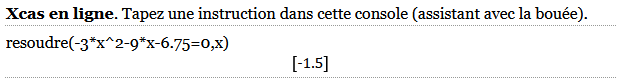
\includegraphics[width=0.9\linewidth]{qf03_q2}
			
			\smallskip
			
			\begin{tikzpicture}
				\tkzTabInit[,lgt=1,espcl=1.15]{$x$/0.6,expr/0.6}{$-\infty$,${-1,5}$,$+\infty$}
				\tkzTabLine{,+,z,-,}
				\only<1>{\draw[] (N22) node[below] {?\vphantom{\scriptsize\faCheckCircle[regular]}};}
				\only<2>{\draw[] (N22) node[below] {\vphantom{?}\vphantom{\scriptsize\faCheckCircle[regular]}};}
			\end{tikzpicture}
			~~~~
			\begin{tikzpicture}
				\tkzTabInit[,lgt=1,espcl=1.15]{$x$/0.6,expr/0.6}{$-\infty$,${-1,5}$,$+\infty$}
				\tkzTabLine{,-,z,-,}
				\only<1>{\draw[] (N22) node[below] {?\vphantom{\scriptsize\faCheckCircle[regular]}};}
				\only<2>{\draw[] (N22) node[below] {\vphantom{?}\red\scriptsize\faCheckCircle[regular]};}
			\end{tikzpicture}
		\end{center}
	\end{block}
	\pause
	\begin{alertblock}{Réponse n°\thediapo}
		On demande à Xcas de résoudre l'équation $-3x^2-9x-6,75=0$, et la racine déterminée ($-1,5$) ainsi que $a=-3\,\ominus$ donnent le signe {\red $\ominus\ominus$}. 
	\end{alertblock}
%	\begin{tikzpicture}
%		\path[overlay,->,>=latex,red,densely dashed,line width=0.75pt](q1a.north) edge[out=110,in=-110] ($(M11)!0.75!(M12)$.south);
%		\path[overlay,blue,densely dotted,line width=0.75pt](q1b.north) edge[out=80,in=-90] ($(M22.south)+(0pt,-30pt)$);
%		\path[overlay,->,>=latex,blue,densely dotted,line width=0.75pt] ($(M22.south)+(0pt,-30pt)$) edge[out=90,in=-90] (N22);
%		\path[overlay,->,>=latex,blue,densely dotted,line width=0.75pt] ($(M22.south)+(0pt,-30pt)$) edge[out=90,in=-90] (N32);
%	\end{tikzpicture}
\end{frame}

%nouvelle diapo
\stepcounter{diapo}
\begin{frame}{\haut{\thediapo}{1}}
	\begin{block}{Question n°\thediapo}
		On donne le tableau de signes d'une fonction $g$.
		\begin{center}
			\begin{tikzpicture}[double distance = 2pt]
				\definecolor{tagada}{RGB}{233,233,243}
				\def\tkzTabDefaultBackgroundColor{tagada}
				\tkzTabInit[espcl=1.25]{$x$/0.6,$g(x)$/0.6}{$-\infty$,$-4$,$0$,$1$,$+\infty$}
				\only<2>{\draw[draw=none,fill=red!25,fill opacity=0.5] (T12) rectangle (N21);}
				\only<2>{\draw[draw=none,fill=red!25,fill opacity=0.5] (N32) rectangle (N41);}
				\tkzTabLine{,+,d,-,z,+,z,-,}
			\end{tikzpicture}
		\end{center}
		L'ensemble des solutions de l'inéquation $g(x)$\noeud{q2a}{\color<2>[rgb]{1,0,0}{$\pg0$}} est :
		\begin{itemize}
			\item $\mathcal{S}=\intervOO{-\infty}{-4} \cup \intervFF{0}{1}$ {\only<1>{?}}{\only<2>{\red\scriptsize\faCheckCircle[regular]}}
			\item $\mathcal{S}=\intervOF{-\infty}{-4} \cup \intervFF{0}{1}$ {\only<1>{?}}
			\item $\mathcal{S}=\intervOF{-4}{0} \cup \intervFO{1}{+\infty}$ {\only<1>{?}}
		\end{itemize}
	\end{block}
	\pause
	\begin{alertblock}{Réponse n°\thediapo}
		Les cases \og {\red $\oplus$} \fg{} et les \og {\red $0$} \fg{} donnent {\red $\mathcal{S}=\intervOO{-\infty}{-4} \cup \intervFF{0}{1}$}.
	\end{alertblock}
	\begin{tikzpicture}
		%\draw[overlay,fill=red!15,fill opacity=0.15] (T12) rectangle (N21);
		%\draw[overlay,fill=red!15,fill opacity=0.15] (N32) rectangle (N41);
		\path[overlay,->,>=Stealth,red,densely dashed,line width=0.75pt](q2a.north) edge[out=90,in=-90] ($(M12)+(0pt,5pt)$);
		\path[overlay,->,>=Stealth,red,densely dashed,line width=0.75pt](q2a.north) edge[out=90,in=-90] ($(M32)+(0,5pt)$);
		\draw[overlay,red,line width=1pt,{Bracket[reversed]}-{Bracket[reversed]}] (T11) -- (N21) ;
		\draw[overlay,red,line width=1pt,{Bracket}-{Bracket}] (N31) -- (N41) ;
	\end{tikzpicture}
\end{frame}

%nouvelle diapo
\stepcounter{diapo}
\begin{frame}{\haut{\thediapo}{3}}
	\begin{block}{Question n°\thediapo}
		On donne des captures d'écran d'une calculatrice.
		\begin{center}
			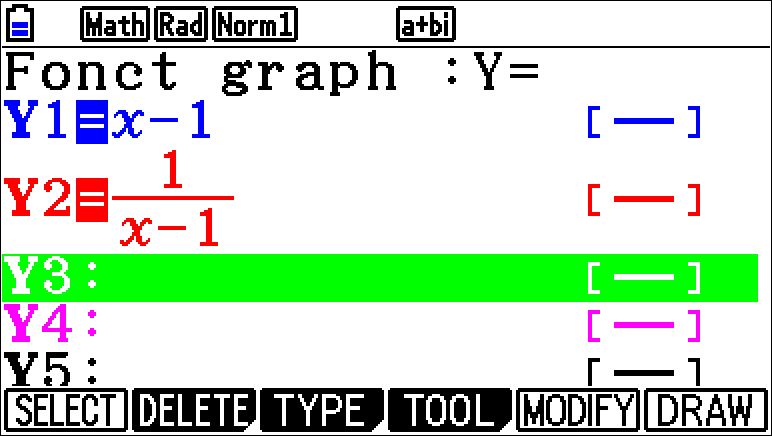
\includegraphics[width=0.25\linewidth]{qf03_q3_a}~~{\only<1>{\noeud{q4b}{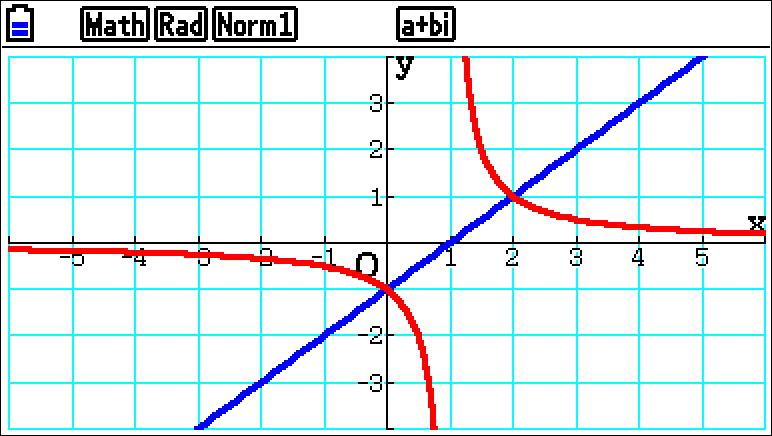
\includegraphics[width=0.25\linewidth]{qf03_q3_b}}}}{\only<2>{\noeud{q4b}{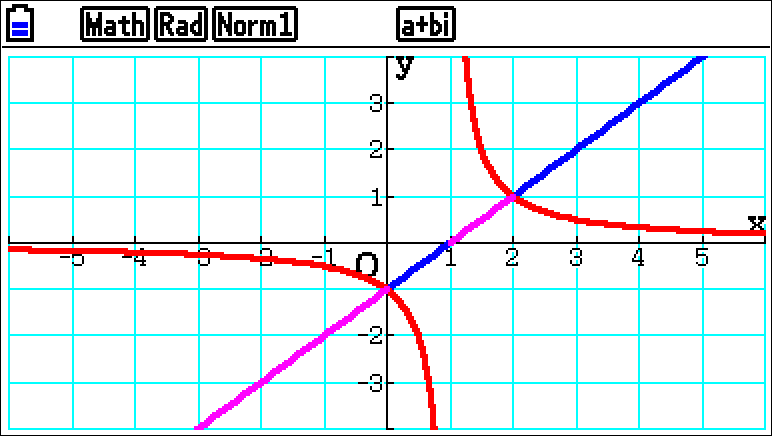
\includegraphics[width=0.25\linewidth]{qf03_q3_c}}}}
		\end{center}
		Les solutions de l'inéquation $x-1 < \dfrac{1}{x-1}$ sont, graphiquement  :
		\begin{itemize}
			\item $\mathcal{S}=\intervOO{-\infty}{0} \cup \intervOO{2}{+\infty}$ {\only<1>{?}}
			\item $\mathcal{S}=\intervOO{0}{2}$ {\only<1>{?}}
			\item $\mathcal{S}=\intervOO{-\infty}{0} \cup \intervOO{1}{2}$ {\only<1>{?}}{\only<2>{\red\scriptsize\faCheckCircle[regular]}}
		\end{itemize}
	\end{block}
	\pause
	\begin{alertblock}{Réponse n°\thediapo}
		Pour résoudre ${\blue x-1} \textcolor{ForestGreen}{<} {\red \dfrac{1}{x-1}}$, on détermine les \noeud{q4a}{\textcolor{Rhodamine}{intervalles}} sur lesquels la {\blue droite} tracée est \textcolor{ForestGreen}{strictement en-dessous} de la {\red courbe}.
		\begin{tikzpicture}
			\path[overlay,Rhodamine,densely dashed,line width=0.75pt] (q4a.north) edge[out=75,in=-50] ($(q4b.south)+(30pt,-10pt)$) ;
			\path[overlay,->,>=Stealth,Rhodamine,densely dashed,line width=0.75pt] ($(q4b.south)+(30pt,-10pt)$) edge[out=130,in=-45] ($(q4b.south)+(-7pt,10pt)$);
			\path[overlay,->,>=Stealth,Rhodamine,densely dashed,line width=0.75pt] ($(q4b.south)+(30pt,-10pt)$) edge[out=130,in=-90] ($(q4b.south)+(10pt,24pt)$);
%			\path[overlay,->,>=Stealth,red,densely dashed,line width=0.75pt](q2a.north) edge[out=90,in=-90] ($(M32)+(0,5pt)$);
%			\draw[overlay,red,line width=1pt,{Bracket[reversed]}-{Bracket[reversed]}] (T11) -- (N21) ;
%			\draw[overlay,red,line width=1pt,{Bracket}-{Bracket}] (N31) -- (N41) ;
		\end{tikzpicture}
	\end{alertblock}
\end{frame}

%nouvelle diapo
\stepcounter{diapo}
\begin{frame}{\haut{\thediapo}{0}}
	\only<1>{\begin{block}{Question\vphantom{p} n°\thediapo}
		\begin{center}
			\begin{tikzpicture}[scale=0.5]
				%logo
				\draw (0,8) node[below right,rotate=15] {
\includegraphics[height=24pt]{grandslam}};
				%grille
				\draw[thick] (6,0) rectangle (12,1) (0,3) rectangle (10,4) (1,5) rectangle (7,6) (6,6) rectangle (14,7) (6,7) rectangle (7,2) (11,8) rectangle (12,0) (14,1) rectangle (15,7);
				%cases
				\foreach \x in {6,7,...,12}
					\draw[thick] (\x,0)--(\x,1);
				\foreach \x in {0,1,...,10}
					\draw[thick] (\x,3)--(\x,4);
				\foreach \x in {1,2,...,7}
					\draw[thick] (\x,5)--(\x,6);
				\foreach \x in {6,7,...,14}
					\draw[thick] (\x,6)--(\x,7);
				\foreach \y in {0,1,...,8}
					\draw[thick] (11,\y)--(12,\y);
				\foreach \y in {2,3,...,6}
					\draw[thick] (14,\y)--(15,\y);
				%labels
				\draw (1,5.5) node[left] {\blue\small\sffamily 1} ;
				\draw (0,3.5) node[left] {\blue\small\sffamily 2} ;
				\draw (6,6.5) node[left] {\blue\small\sffamily 3} ;
				\draw (6,0.5) node[left] {\blue\small\sffamily 4} ;
				\draw (6.5,7) node[above] {\red\small\sffamily 1} ;
				\draw (11.5,8) node[above] {\red\small\sffamily 2} ;
				\draw (14.5,7) node[above] {\red\small\sffamily 3} ;
				%indices
				\draw (-1,-1) node[right] {\blue\small\sffamily 1 : Annule une fonction} ;
				\draw (-1,-2) node[right] {\blue\small\sffamily 2 : Peut se résoudre avec un tds} ;
				\draw (-1,-3) node[right] {\blue\small\sffamily 3 : Utile pour la pente} ;
				\draw (-1,-4) node[right] {\blue\small\sffamily 4 : Courbe du 1\up{er} degré} ;
				\draw (9,-1) node[right] {\red\small\sffamily 1 : Très utile pour le 2\up{d} degré} ;
				\draw (9,-2) node[right] {\red\small\sffamily 2 : Courbe du  2\up{d} degré} ;
				\draw (9,-3) node[right] {\red\small\sffamily 3 : \og Extremum \fg{} d'une courbe} ;
				\draw (9,-4) node[right] {\red\small\sffamily \phantom{3 :} du 2\up{d} degré} ;
			\end{tikzpicture}
		\end{center}
	\end{block}}
	\pause
	\only<2>{\begin{alertblock}{Réponse n°\thediapo}
		\begin{center}
			\begin{tikzpicture}[scale=0.5]
				%logo
				\draw (0,8) node[below right,rotate=15] {
\includegraphics[height=24pt]{grandslam}};
				%grille
				\draw[thick] (6,0) rectangle (12,1) (0,3) rectangle (10,4) (1,5) rectangle (7,6) (6,6) rectangle (14,7) (6,7) rectangle (7,2) (11,8) rectangle (12,0) (14,1) rectangle (15,7);
				%cases
				\foreach \x in {6,7,...,12}
					\draw[thick] (\x,0)--(\x,1);
				\foreach \x in {0,1,...,10}
					\draw[thick] (\x,3)--(\x,4);
				\foreach \x in {1,2,...,7}
					\draw[thick] (\x,5)--(\x,6);
				\foreach \x in {6,7,...,14}
					\draw[thick] (\x,6)--(\x,7);
				\foreach \y in {0,1,...,8}
					\draw[thick] (11,\y)--(12,\y);
				\foreach \y in {2,3,...,6}
					\draw[thick] (14,\y)--(15,\y);
				%labels
				\draw (1,5.5) node[left] {\blue\small\sffamily 1} ;
				\draw (0,3.5) node[left] {\blue\small\sffamily 2} ;
				\draw (6,6.5) node[left] {\blue\small\sffamily 3} ;
				\draw (6,0.5) node[left] {\blue\small\sffamily 4} ;
				\draw (6.5,7) node[above] {\red\small\sffamily 1} ;
				\draw (11.5,8) node[above] {\red\small\sffamily 2} ;
				\draw (14.5,7) node[above] {\red\small\sffamily 3} ;
				%indices
				\draw (-1,-1) node[right] {\blue\small\sffamily 1 : Annule une fonction} ;
				\draw (-1,-2) node[right] {\blue\small\sffamily 2 : Peut se résoudre avec un tds} ;
				\draw (-1,-3) node[right] {\blue\small\sffamily 3 : Utile pour la pente} ;
				\draw (-1,-4) node[right] {\blue\small\sffamily 4 : Courbe du 1\up{er} degré} ;
				\draw (9,-1) node[right] {\red\small\sffamily 1 : Très utile pour le 2\up{d} degré} ;
				\draw (9,-2) node[right] {\red\small\sffamily 2 : Courbe du  2\up{d} degré} ;
				\draw (9,-3) node[right] {\red\small\sffamily 3 : \og Extremum \fg{} d'une courbe} ;
				\draw (9,-4) node[right] {\red\small\sffamily \phantom{3 :} du 2\up{d} degré} ;
				%SOLUTIONS
				\foreach \lettre/\X in {D/6,R/7,O/8,I/9,T/10,E/11}{\draw ({\X+0.5},0.5) node {\small\sffamily \lettre};}
				\foreach \lettre/\X in {D/6,E/7,C/8,A/9,L/10,A/11,G/12,E/13}{\draw ({\X+0.5},6.5) node {\small\sffamily \lettre};}
				\foreach \lettre/\X in {I/0,N/1,E/2,Q/3,U/4,A/5,T/6,I/7,O/8,N/9}{\draw ({\X+0.5},3.5) node {\small\sffamily \lettre};}
				\foreach \lettre/\X in {R/1,A/2,C/3,I/4,N/5,E/6}{\draw ({\X+0.5},5.5) node {\small\sffamily \lettre};}
				\foreach \lettre/\Y in {D/6,E/5,L/4,T/3,A/2}{\draw (6.5,{\Y+0.5}) node {\small\sffamily \lettre};}
				\foreach \lettre/\Y in {P/7,A/6,R/5,A/4,B/3,O/2,L/1,E/0}{\draw (11.5,{\Y+0.5}) node {\small\sffamily \lettre};}
				\foreach \lettre/\Y in {S/6,O/5,M/4,M/3,E/2,T/1}{\draw (14.5,{\Y+0.5}) node {\small\sffamily \lettre};}
			\end{tikzpicture}
		\end{center}
	\end{alertblock}}
\end{frame}

\end{document}